\begin{appendices}
    \crefalias{section}{appsec}
    \chapter{Implementation} \label{app:Implementation}
    The code can be found here[]. \\
    Both the Identification and the Pricing Problem were programmed in Python 2.7 using NumPy 1.12.1, SciPy 0.19.1 and Pytorch 0.1.12 modules [web cites] \cite{SCPOptimizeDocs}\cite{NPDocs}. [Results from Python plotted in Matplotlib 2.0.2] With some code optimizations, the input dataset $\matr{F}$ was built using NumPy's \texttt{ndarray} and Pytorch's \texttt{tensor} functions. Since Pytorch offers NumPy-like code base but with dedicated neural network functions and submodules, Pytorch's \texttt{relu} and \texttt{softmax} functions were used along with other matrix operations.\\
    
    \section{Specific Implementation Details for the Pricing Problem}
    Among all the code optimizations in both models, some in that for the Pricing Problem are worth discussing, as they drastically differ from Algorithm \ref{alg:Solving the Pricing Problem} or are intricate. Most optimizations relevant to the Identification Problem are trivial and relate directly to those for the Pricing Problem. Therefore, only those in the Pricing Problem model are discussed.
    
    \subsection{Building the Dataset $\matr{F}$}
    Notice that we build the dataset $\matr{F}$ and batch-multiply it with $\matr{w_1}$ on each iteration/epoch (lines 2-3 of Algorithm \ref{alg:Solving the Pricing Problem}). Doing these steps are repetitive as most elements of $\matr{F}$, distances $\matr{D}$ and environmental feature vector $\vect{f}$, do not change unlike rewards $\vect{r}$. Moreover since $\matr{w_1}$ is fixed, Algorithm \ref{alg:Solving the Pricing Problem} would repetitively multiply the $\vect{f}$ and $\matr{D}$ components of $\matr{F}$ with $\matr{w_1}$. To avoid these unnecessary computations, we preprocessed most of $\matr{F}$ by batch-multiplying with $\matr{w_1}$ and only multiplied $\vect{r}$ with the corresponding elements of $\matr{w_1}$. Figure \ref{fig:Splitting and Batch Multiplying F and w1} describes the process graphically.\\
    \begin{figure}[!htbp]
        \centering
        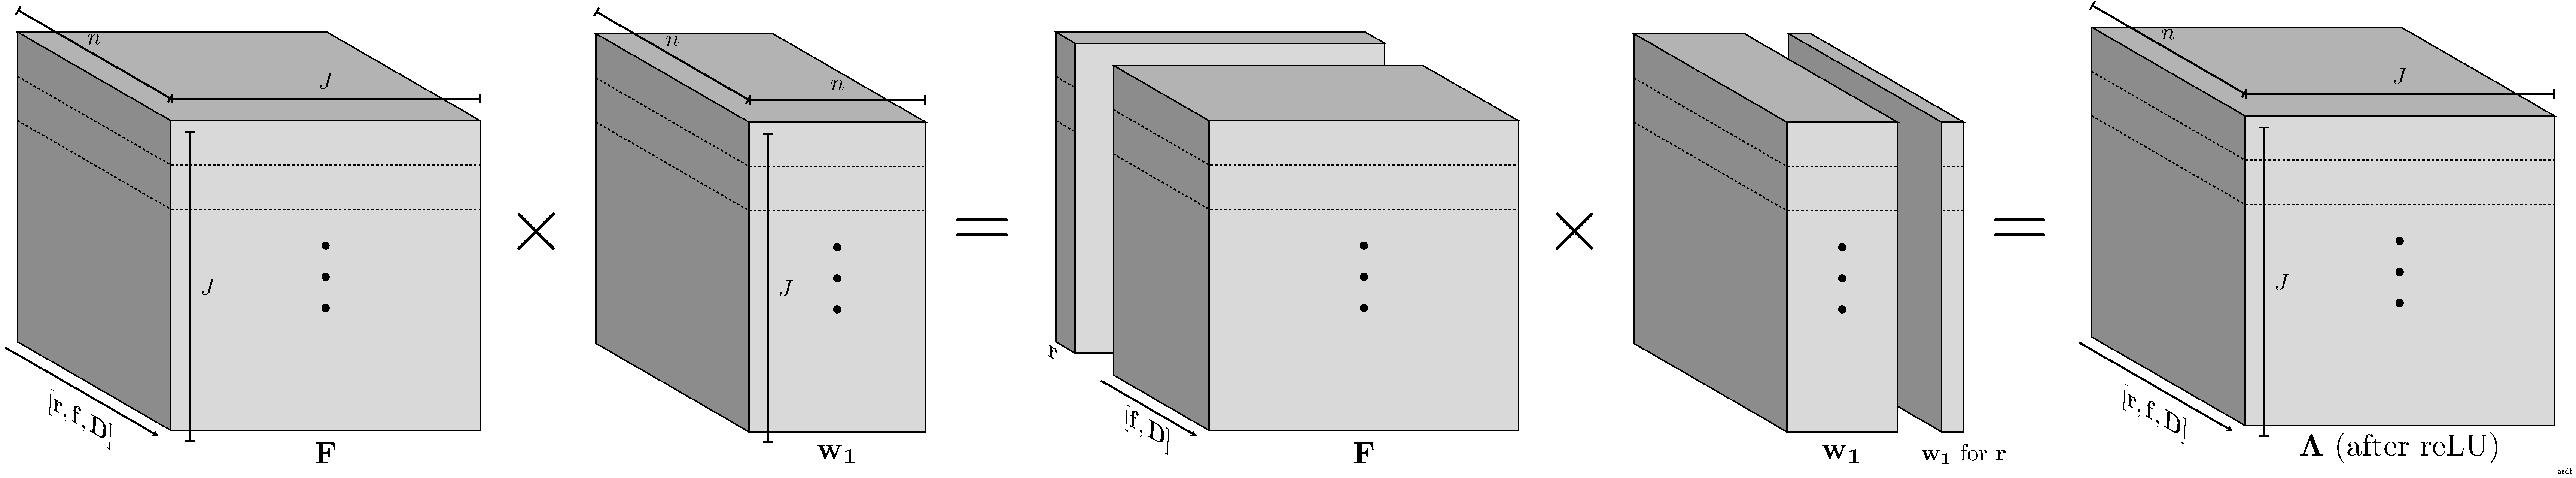
\includegraphics[width=\linewidth]{split_and_batch_multiply}
        \caption{Splitting and Batch Multiplying $\matr{F}$ and $\matr{w_1}$}
        \label{fig:Splitting and Batch Multiplying F and w1}
    \end{figure}    
    Although this preprocessing might seem applicable for the model in Identification Problem too, it does not apply fully. Since the weights $\matr{w_1}$ are updated on each iteration/epoch, we cannot multiply them with parts of $\matr{F}$ beforehand (Algorithm \ref{alg:Algorithm for the Identification Problem}). However, we can combine $\matr{D}$ and $\vect{f}$ in the preprocessing stage and simply append $\vect{r}[t]$ on each iteration, saving computation time.
    
    \subsection{Modeling the Linear Programming Problem in the Standard Format}
    The \texttt{scipy.optimize} module's \texttt{linprog} function requires that the arguments are in standard LP format. As discussed in \cref{sec:Calculating Rewards}, Equation \ref{eqn:lp_code_constrain_rewards} resembles the standard format more closely than \ref{eqn:lp_math_constrain_rewards}, but it may not be clear how so.\\
    
    Considering $\vect{u}$ and $\vect{r'}$ as variables $\vect{x}$, Equation \ref{eqn:lp_code_constrain_rewards} translates into Equation \ref{eqn:lp_matrix_rewards} ($J$ is the number of locations).
    \begin{equation} \label{eqn:lp_matrix_rewards}
    \begin{aligned}
    & \text{minimize}
    & & \begin{bmatrix}
    \vect{0_J}\\
    \vect{1_J}\\
    \end{bmatrix}^T
    \begin{bmatrix}
    \vect{r'}\\
    \vect{u}
    \end{bmatrix}\\ \\
    & \text{subject to}
    & & \begin{bmatrix}
    I_J & -I_J\\
    -I_J & -I_J\\
    \vect{1}^T_J & \vect{0}^T_J\\
    \end{bmatrix}
    \begin{bmatrix}
    \vect{r'}\\
    \vect{u}\\
    \end{bmatrix} \leq
    \begin{bmatrix}
    \vect{r}\\
    -\vect{r}\\
    \mathcal{R}\\
    \end{bmatrix}\\
    &&& r'_i, u_i \geq 0
    \end{aligned}
    \end{equation}
    
    \chapter{GPU Speedup in LP Computation} \label{app:GPU Speedup in LP Computation}
    Even though we intentionally transferred the rewards vector to and constrained it using \texttt{scipy.optimize} module's \texttt{linprog} function on the CPU, we obtained an unexpected GPU Speedup in the LP runtimes (see \cref{sec:PriProbRes - GPU} and Figure \ref{fig:Finding Rewards - Time taken by the LP}). Confounded by this weird behavior, we wanted to pinpoint the reason(s). It was clear that \texttt{scipy.optimize.linprog()} could not have differentiated between the configurations and delivered different results. However, since this was not our study's prime motive, we did not take a strong quantitative approach in determining the cause(s).
    
    \section{Possible Reasons for GPU Speedup} \label{app:Possible Reasons for GPU Speedup}
    There could have been many reasons for this bizarre behavior, including but not limited to:
    \begin{enumerate}
        \item SciPy's Optimize module differentiating between configurations. This can be ruled out because the module could not have known the configuration during which it was called. This is because only Pytorch's tensors were executable on the GPU, whereas NumPy tensors were only operable on the CPU\footnote{We didn't mind SciPy.Optimize using MKL, BLAS or any other linear algebra libraries. Even if it had, there wouldn't be a distinction between CPU and GPU ``set'' configurations!} \cite{PTDocs,NPDocs,SCPOptimizeDocs}. SciPy's Optimize Module identifying the configurations is just supernatural.
        \item CPU ``set'' exploiting more main memory than GPU ``set''. We suspected that since CPU ``set'' configuration's operations were executed solely on the CPU, the residing datasets could have used more main memory than when GPU ``set'' was running. This could have hampered the performance of LP with CPU ``set'', as the LP had lesser space to operate in. Unlike the 1\textsuperscript{st} possibility, this would have meant that CPU ``set'' was slowing down the LP, and not that GPU ``set'' was speeding up the LP.
        \item Neural network in CPU ``set'' using more CPU threads than that in GPU ``set''. The Intel i7-7700K processor is quad-core with 8 threads. Since Pytorch uses OpenMP \cite{PTDocs,OpenMP}, a parallel processing API for CPUs, we fancied the neural network to run on simultaneous processors/threads, thus allowing less available threads for the LP to run/taking up CPU's resources/causing latency due to synchronization locks\footnote{\Cref{alg:Solving the Pricing Problem} for the Pricing Problem is sequential in that calculated tensors have to be fully available before LP starts - a `Fork and Join' synchronization task \cite[Section 2.2]{IssuesMP}.}.
    \end{enumerate}

    \section{LP Slowing Down or Speeding Up?} \label{app:LP Slowing Down or Speeding Up?}
    First we determined whether the LP runtime was being sped up in GPU ``set'' or slowed down in CPU ``set''. To test this, we created a copy of our Pricing Problem's model, which focused only on logging LP runtimes at each epoch. For a baseline comparison, we scripted the same LP without the neural network, which gave us the \underline{true} runtimes for the LP (`Only LP' setting), without any involvement of Pytorch modules or functions. 
    
    Comparing the former runtimes (CPU and GPU ``set'') with `Only LP' runtime, we observed that the LP in the CPU ``set'' configuration took longer to execute than that in `Only LP' setting during each epoch (\Cref{fig:LP Runtime Example for Different Configurations}). We also noticed little to no interaction between the neural network in GPU ``set'' with the LP, as the runtimes of LP in GPU ``set'' were similar to those of LP in `Only LP' setting. This confirmed that CPU ``set'' was slowing down the LP and GPU ``set'' was not speeding it up. But why?
    \begin{figure}[!htbp]
        \centering
        \begin{tikzpicture}
        \begin{axis}[
            width=\textwidth,
            height=8cm,
            xlabel=Epochs,
            ylabel=Time/s,
            scaled y ticks = false,
            grid=both,
            every axis plot/.append style={very thick},
        ]
        \addplot[red] table [col sep=comma,x=epoch, y=cpuset]{datafiles/lp_time_logs.csv};
        \addlegendentry{CPU ``set''}
        
        \addplot[blue] table [col sep=comma,x=epoch, y=gpuset]{datafiles/lp_time_logs.csv};
        \addlegendentry{GPU ``set''}
        
        \addplot[brown] table [col sep=comma,x=epoch, y=onlylp]{datafiles/lp_time_logs.csv};
        \addlegendentry{`Only LP'}
        
        \end{axis}
        \end{tikzpicture}
        \caption[LP Runtime Example for Different Configurations]{LP Runtime Example for Different Configurations: LPs in both CPU and GPU ``set'' start running slowly, but pick up speed after $\approx$ 20 epochs. A possible reason for spikes in CPU ``set'' is given in []. The test was done on a random dataset for 200 epochs, while the other experiment specifications were same as in \cref{sec:Experiment Specifications}.}
        \label{fig:LP Runtime Example for Different Configurations}
    \end{figure}
    
    \section{CPU and Main Memory Usage} \label{app:CPU and Main Memory Usage}
    While logging the LP runtimes in \Cref{app:LP Slowing Down or Speeding Up?}, we also recorded an estimate of the amount of computer resources both configurations were using. Using the \texttt{top} package in Ubuntu, we polled the resource monitor every 0.1 seconds while the python script was running\footnote{\label{foo:logs not epochs} Running processes were polled every 0.1 seconds - contributing to a `log'. The longer the script ran, the more logs collected.}. \Cref{fig:CPU Usage by Different Configurations,fig:Main Memory Usage by Different Configurations} shows how much main memory and CPU resource each setting was using.
    
    \subsection{CPU Usage}
    We see that CPU ``set'' constantly used more than 4 out of 8 available threads during execution, i.e., $>400\%$ CPU usage, while GPU ``set'' only used a single thread. Also, since we polled at every 0.1 second, and the LP took a minimum of 0.14 seconds (\Cref{fig:LP Runtime Example for Different Configurations}), the data plotted in \Cref{fig:CPU Usage by Different Configurations} must show resource use \textit{while} the LP was running. Considering that the LP in `Only LP' setting only used a single thread ($100\%$), it makes sense that GPU ``set'' would use 1 thread for execution - the neural network operations were performed on the GPU, leaving the CPU empty for management and LP. 
    \begin{figure}[!htbp]
        \centering
        \begin{minipage}{.49\textwidth}
            \centering
            \begin{tikzpicture}
            \begin{axis}[
            name=cpuusage-cpuset,
            width=\textwidth,
            enlarge x limits=0.15,
            no markers,
            ymax=800,
            ymin=0,
            ]
            \addplot+[fill=red, opacity=.4] table [col sep=comma,x=epoch, y=cpu]{datafiles/ext_cpu_cpuset.csv} \closedcycle;
            
            \addplot+[very thick, red!50!black] table [col sep=comma,x=epoch, y=cpu]{datafiles/ext_cpu_cpuset.csv};
            
            \end{axis}
            
            \begin{axis}[
            name=cpuusage-gpuset,
            at=(cpuusage-cpuset.below south west), anchor=above north west,
            width=\textwidth,
            enlarge x limits=0.15,
            no markers,
            ylabel={CPU Usage/\%},
            ymax=200,
            ymin=0,
            ]
            \addplot+[fill=blue, opacity=.4] table [col sep=comma,x=epoch, y=cpu]{datafiles/ext_cpu_gpuset.csv} \closedcycle;
            
            \addplot+[very thick, blue!50!black] table [col sep=comma,x=epoch, y=cpu]{datafiles/ext_cpu_gpuset.csv};
            \end{axis}
            
            \begin{axis}[
            name=cpuusage-onlylp,
            at=(cpuusage-gpuset.below south west), anchor=above north west,
            width=\textwidth,
            enlarge x limits=0.15,
            no markers,
            xlabel={Logs},
            ymax=200,
            ymin=0,
            ]
            \addplot+[fill=green, opacity=.4] table [col sep=comma,x=epoch, y=cpu]{datafiles/ext_onlylp.csv} \closedcycle;
            
            \addplot+[very thick, green!50!black] table [col sep=comma,x=epoch, y=cpu]{datafiles/ext_onlylp.csv};
            \end{axis}
            \end{tikzpicture}
            \caption[CPU Usage by Different Configurations]{CPU Usage by Different Configurations\textsuperscript{\ref{foo:logs not epochs}}: From top - CPU ``set'', GPU ``set'', `Only LP'. CPU Usage for GPU ``set'' and `Only LP' are very similar as operations other than the LP run on the GPU.}
            \label{fig:CPU Usage by Different Configurations}
        \end{minipage}\hfill
        \begin{minipage}{.49\textwidth}
            \centering
            \begin{tikzpicture}
            \begin{axis}[
            name=memusage-cpuset,
            width=\textwidth,
            enlarge x limits=0.15,
            no markers,
            ymax=1,
            ymin=0,
            ]
            \addplot+[fill=red, opacity=.4] table [col sep=comma,x=epoch, y=mem]{datafiles/ext_cpu_cpuset.csv} \closedcycle;
            
            \addplot+[very thick, red!50!black] table [col sep=comma,x=epoch, y=mem]{datafiles/ext_cpu_cpuset.csv};
            
            \end{axis}
            
            \begin{axis}[
            name=memusage-gpuset,
            at=(memusage-cpuset.below south west), anchor=above north west,
            width=\textwidth,
            enlarge x limits=0.15,
            no markers,
            ylabel={Main Memory Usage/\%},
            ymax=10,
            ymin=0,
            ]
            \addplot+[fill=blue, opacity=.4] table [col sep=comma,x=epoch, y=mem]{datafiles/ext_cpu_gpuset.csv} \closedcycle;
            
            \addplot+[very thick, blue!50!black] table [col sep=comma,x=epoch, y=mem]{datafiles/ext_cpu_gpuset.csv};
            \end{axis}
            
            \begin{axis}[
            name=memusage-onlylp,
            at=(memusage-gpuset.below south west), anchor=above north west,
            width=\textwidth,
            enlarge x limits=0.15,
            no markers,
            xlabel={Logs},
            ymax=1,
            ymin=0,
            ]
            \addplot+[fill=green, opacity=.4] table [col sep=comma,x=epoch, y=mem]{datafiles/ext_onlylp.csv} \closedcycle;
            
            \addplot+[very thick, green!50!black] table [col sep=comma,x=epoch, y=mem]{datafiles/ext_onlylp.csv};
            \end{axis}
            \end{tikzpicture}
            \caption[Main Memory Usage by Different Configurations]{Main Memory Usage by Different Configurations\textsuperscript{\ref{foo:logs not epochs}}: From top - CPU ``set'', GPU ``set'', `Only LP'. The neural network doesn't occupy much main memory in CPU ``set'' - could be due to Python/Pytorch's garbage collection.}
            \label{fig:Main Memory Usage by Different Configurations}
        \end{minipage}
    \end{figure}

    On the other hand, it is apparent that CPU ``set'' had multi-threaded operations running simultaneously (\#3 in \Cref{app:Possible Reasons for GPU Speedup}). Since we know from the `Only LP' setting that the LP only used a single thread, the other threads in CPU ``set'' must have been the neural network. Although this counters our reasoning that the neural network threads should have fully synchronized and terminated before the LP started, it seems that those threads were still active. Therefore, Pytorch and OpenMP continued calculating for the neural network even after the LP had started. Nevertheless, this activity does not impact correctness, as found from optimization tests on CPU ``set''\footnote{CPU ``set'' tests were done for optimization on original datasets to check this. Since we got the same results as for GPU ``set'' optimization tests \Cref{sec:PriProbRes - Optimization}, the results are not shown in the report.} (same optimization figures as obtained for GPU ``set'' - \Cref{sec:PriProbRes - Optimization}).
    
    \subsection{Main Memory Usage}
    GPU ``set'' was using 10 times as much main memory as CPU ``set'' or `Only LP', in addition to storing and operating on tensors in the GPU's internal memory. Not only this is weird, but it is also opposite of what we expected to happen - CPU ``set'' using more main memory and hampering LP performance. It is ironic that the LP performs better (even as good as `Only LP') on GPU ``set'' even when the configuration uses a lot more main memory than CPU ``set''. Clearly, main memory usage cannot be a criterion for assessing LP performance on different configurations.
    
    \section{Parallelism Doesn't Always Help: Thread Synchronization Delays} \label{app:Parallelism Doesn't Always Help}
    Now that we had determined that multi-processing/threading might be the root of the strange GPU Speedup, we asked why. Were the simultaneous threads gobbling up valuable CPU resources or were the neural network threads causing latency due to prolonged process synchronization?
    
    Testing the first possibility was trivial enough - manually run LPs simultaneously on different threads (in 4 available hyper-threaded cores) and see if they impact each other's performance. If they didn't, multi-threading would prove independent in terms of CPU resources, and there would be no reason to believe that simultaneous threads would eat up each other's CPU resources. Running several instances of the LP on multiple threads and cores, we found no impact of multi-processed scripts on each other when it came to CPU resources. The scripts were unaffected by any other processes on other cores of CPU. One might very well argue that the independence of the LPs in these tests does not highlight the dependence of the LP to neural network in the Pricing Problem, and that these tests are wrongly based. Well, we contend that the argument pertains to the second possibility and not the first one. 
    
    CPU ``set'' was utilizing more than half of the available 8 threads, and we were concerned if there was latency due to thread synchronization. Since we used \texttt{scipy.optimize.linprog()}'s Simplex solver, which was distinct from Pytorch, this led to a `Fork and Join' task-synchronization requirement \cite[Section 2.2]{IssuesMP} after the neural network was complete. We suspected this causing latency as the LP waited for the neural network to finish. To test this hunch, we ran the scripts with restricted access to CPU threads. Using the \texttt{taskset} command in Ubuntu, we manually forced the script to use specific CPU threads. If CPU ``set'' slowed down even after restriction, then there would not been synchronization delays - the script wasn't heavily threaded. Whereas, a gradual increase in execution time with the number of available threads would show that more threads for the neural network create delays in LP's execution.
    \begin{figure}[!htbp]
        \centering
        \begin{tikzpicture}
        \begin{axis}[
        width=\textwidth,
        height=8cm,
        xlabel=Epochs,
        ylabel=Time/s,
        scaled y ticks = false,
        grid=both,
        every axis plot/.append style={very thick},
        ]
        \addplot[red] table [col sep=comma,x=epoch, y=t1]{datafiles/lp_time_logs_threads.csv};
        \addlegendentry{1 Thread}
        
        \addplot[blue] table [col sep=comma,x=epoch, y=t3]{datafiles/lp_time_logs_threads.csv};
        \addlegendentry{3 Threads}
        
        \addplot[brown] table [col sep=comma,x=epoch, y=t5]{datafiles/lp_time_logs_threads.csv};
        \addlegendentry{5 Threads}
        
        \addplot[black] table [col sep=comma,x=epoch, y=t7]{datafiles/lp_time_logs_threads.csv};
        \addlegendentry{7 Threads}
        
        \end{axis}
        \end{tikzpicture}
        \caption[LP Runtime Example with Restricted Thread Access]{LP Runtime Example with Restricted Thread Access: With only 1 thread accessible to the whole script (neural network and LP), the LP performs as good as `Only LP' setting (\Cref{app:LP Slowing Down or Speeding Up?}). We start seeing erratic synchronization delays for 3 threads, and constant delays with more threads.}
        \label{fig:LP Runtime Example with Restricted Thread Access}
    \end{figure}
    
    \Cref{fig:LP Runtime Example with Restricted Thread Access} shows how the access to CPU's threads affected the LP's runtime. Clearly, restricting access to a single thread avoids synchronization delays in the Fork and Join task, allowing the LP to run faster on all epochs. Based on this finding, we restricted the Pricing Problem model's access to the all CPU threads, giving us better CPU ``set'' performance (\Cref{sec:PriProbRes - GPU}) and removing the unexpected GPU Speedup (\Cref{fig:Restricted Finding Rewards - Time taken by the LP,fig:Restricted Finding Rewards - Speedup for LP}).
    \begin{figure}[!htbp]
        \centering
        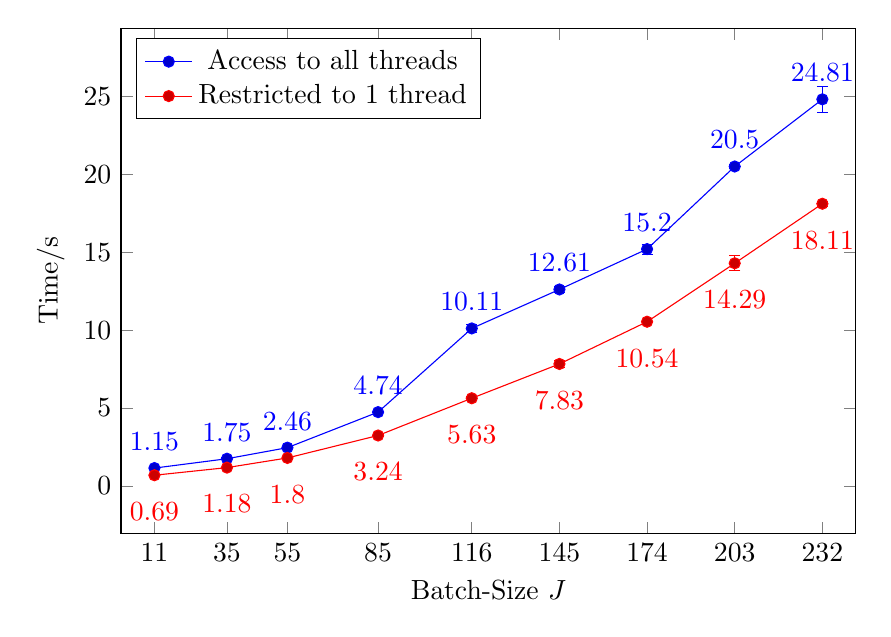
\begin{tikzpicture}
        \begin{axis}[
        width=.9\textwidth,
        height=8cm,
        xtick=data,
        xlabel={Batch-Size $J$},
        ylabel={Time/s},
        enlarge y limits=0.15,
        enlarge x limits=0.05,
        y tick label style={/pgf/number format/1000 sep=},
        extra y tick style={grid=major, tick label style={xshift=-1cm}},
        legend style={at={(0.02,.98)},
            anchor=north west},
        nodes near coords,
        every node near coord/.append style={yshift=-0.7cm}
        ]
        \addplot+ [mark=*,
        nodes near coords=\raisebox{0.8cm}{\pgfmathprintnumber\pgfplotspointmeta},error bars/.cd, y dir=both,y explicit
        ] coordinates {
            (11,1.15) +- (0.10,0.10)
            (35,1.75) +- (0.05,0.05)
            (55,2.46) +- (0.01,0.01)
            (85,4.74) +- (0.03,0.03)
            (116,10.11) +- (0.26,0.26)
            (145,12.61) +- (0.20,0.20)
            (174,15.20) +- (0.32,0.32)
            (203,20.50) +- (0.15,0.15)
            (232,24.81) +- (0.82,0.82)
        };  % no restriction
        \addplot+ [mark=*,error bars/.cd, y dir=both,y explicit] coordinates {
            (11,0.69) +- (0.004,0.004)
            (35,1.18) +- (0.002,0.002)
            (55,1.80) +- (0.01,0.01)
            (85,3.24) +- (0.03,0.03)
            (116,5.63) +- (0.14,0.14)
            (145,7.83) +- (0.22,0.22)
            (174,10.54) +- (0.03,0.03)
            (203,14.29) +- (0.48,0.48)
            (232,18.11) +- (0.17,0.17)
        };  % restricted to 1thread
        \legend{Access to all threads,Restricted to 1 thread}
        \end{axis}
        \end{tikzpicture}
        \caption[Neural Network's Performance (CPU ``set'') with and without Thread Access Restrictions]{Neural Network's Performance (CPU ``set'') with and without Thread Access Restrictions: Data from the Pricing Problem Tests in \Cref{sec:PriProbRes - GPU}. Contrary to one's expectation, fewer threads decreases the network's execution time.}
        \label{fig:Neural Network's Performance (CPU ``set'') with and without Thread Access Restrictions}
    \end{figure}

    Well, does it reduce the neural network's performance (higher runtime due to lower parallelism)? Shockingly, it does the opposite: increase the performance. Explaining this phenomena requires in-depth understanding of Pytorch's implementation with OpenMP, but there can be some possibilities:
    \begin{itemize}
        \item More parallelism could result in competition between threads for Main Memory access \cite[Section 2.1]{IssuesMP}.
        \item There could still be inconspicuous synchronization requirements in the network, caused due to our algorithm's structure.
    \end{itemize}
    We cannot ensure one of them nor deny any other possibility. This area requires further research and we are open to suggestions. As for the results, we use the restricted access results for CPU ``set'' to calculate GPU Speedups in \Cref{sec:PriProbRes - Optimization}.
\end{appendices}